\documentclass[a4paper]{article} %%% use \documentstyle for old LaTeX compilers

\usepackage[portuguese]{babel} %%% 'french', 'german', 'spanish', 'danish', etc.
\usepackage{makeidx}
\usepackage{multirow}
\usepackage{multicol}
\usepackage[dvipsnames,svgnames,table]{xcolor}
\usepackage[dvips]{graphicx} 
\usepackage[utf8x]{inputenc}
\usepackage{epstopdf}
\usepackage{ulem}
\usepackage{hyperref}
\usepackage{amsmath}
\usepackage{amssymb}
\usepackage{txfonts}
\usepackage{mathdots}
\usepackage[classicReIm]{kpfonts}

% You can include more LaTeX packages here 

\usepackage[a4paper,top=2.5cm,bottom=2.5cm,left=3cm,right=3cm,marginparwidth=1.75cm]{geometry}

\begin{document}

%\selectlanguage{english} %%% remove comment delimiter ('%') and select language if required

\title{Kepler's laws}
\author{Bruno da silva}

\fontfamily{phv}\selectfont
\begin{titlepage}
	\begin{center}
		{\scshape\Large Universidade Federal Fluminense -UFF \par}
		\vspace{7cm}
		{\huge\bfseries Leis de Kepler \par}
		\vspace{5.5cm}
		{\itshape Autor Bruno da Silva Machado \par}      
			
		\vspace{6.5cm}    
			
		\vfill
		{\large \today\par}
	\end{center}
\end{titlepage}

\setcounter{secnumdepth}{0}
\section{Introdu\c{c}\~{a}o}
\noindent

O movimento planet\'{a}rio \'{e} o movimento que os planeta fazem ao redor de uma estrela este movimento obedecem as leis de Kepler, que por sua v\^{e}z podem ser obtidas pelas leis de Newton

As leis do movimento planet\'{a}rio \'e um dos maiores \^{e}xitos intelectuais do seculo 16 e 17 convenceram a comunidade científica da \'{e}poca sobre a realidade do modelo heliocêntrico, que afirmava que a Terra girava em torno do Sol.

Neste trabalho vamos estudar melhor este tipo de movimento analisar algumas de suas caracter\'{i}sticas atrav\'{e}s do m\'{e}todo num\'{e}rico que \'{e} um m\'{e}todo para solucionar equa\c{c}\~{o}es diferenciais ordin\'{a}rias de primeira ordem com um valor inicial previamente informado. \'{E} o tipo mais simples de m\'{e}todo expl\'{i}cito para integra\c{c}\~{a}o num\'{e}rica para equa\c{c}\~{o}es diferenciais ordin\'{a}rias.
\noindent \eject 

\section{3° lei de Kepler}
\noindent 

Um parâmetro importante do movimento circular é seu período. Lembre-se de que o período T é o tempo necessário para completar uma órbita. A relação entre velocidade, raio e período é:
\[v = \frac{circunferencia}{per\acute{i}odo} = \frac{2\pi r}{T} \]

\begin{center}
	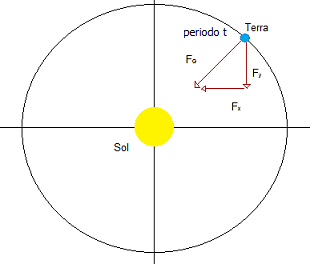
\includegraphics[width=3.10in,height=2.64in,keepaspectratio = false]{image2.png}
	
	\scriptsize Figura 1. Terra girando ao redor do sol a força gravitacional $F_g$ exerce força que mantem o planeta orbitando e um agente responsável pelo período da terra. 
	
\end{center}

A figura 1 acima mostra um corpo de grande massa M, como a Terra ou o Sol, e um corpo mais leve m em sua órbita. O corpo mais leve será chamado de satélite, mesmo que seja um planeta em órbita do Sol. A segunda lei de Newton para o satélite é
\[F_{M em m} = \frac{GMm}{r^2} = ma_r = \frac{mv^2}{r}\]
Dessa forma, o módulo da velocidade de um satélite numa órbita circular é:
\[v = \sqrt{\frac{GM}{r}}\]

Podemos encontra uma relação entre o período de um planeta e o raio de sua orbita usando a equação anterior
\[\frac{2\pi{r}}{T} = \sqrt{\frac{GM}{r}}\]

Elevando ao  quadrado os dois lados da equação ee isolando T, obtemos:
\begin{equation}
	T^2 = \left(\frac{4\pi^2}{GM}\right)r^3
\end{equation}

em outras palavras, o quadrado do período de revolução de cada planeta em torno do sol é diretamente proporcional ao cubo da distância média desse planeta ao Sol.
A terceira lei de Kepler pode matematicamente ser descrita de maneira simplificada pela equação abaixo:
\[T^2 = Kr^3\]

Onde:
\begin{enumerate}
	\item T = período de revolução
	\item K = constante de proporcionalidade que equivale a $\left(\frac{4\pi^2}{GM}\right)$
	\item r = a distancia da Terra ao Sol (semieixo)
\end{enumerate}

Quanto maior o semieixo, maior o período, ou seja, maior o ano do planeta.
Além de confirmarem as teorias de Copérnico, as Leis de Kepler mostraram a representação precisa da órbita dos planetas, ou seja, elipses quase circulares.
Também são válidas para qualquer corpo que gravite em torno de outro com massa muito maior, como os satélites artificiais que se movem em torno da Terra.

A Tabela a seguir contém informações astronômicas sobre o Sol, a Terra, a Lua e outros planetas do Sistema Solar. Podemos usar esses dados para verificar a validade da Equação (1). A figura seguir é um gráfico de log T versus log r para todos os planetas da Tabela, Note que as escalas de cada eixo aumentam logaritmicamente - por fatores de 10 – em vez de linearmente. Como podemos ver, o gráfico resultante é uma linha reta

\begin{table}
	\centering
	\begin{tabular}{l|c|r}
		Planeta & T(anos) & r (UA) \\\hline
		Mercúrio & 0.241 & 0.387 \\
		Vênus & 0.615  & 0.723\\
		Terra & 1 & 1\\
		Marte & 1.88 & 1.523\\
		Júpiter & 11.86 & 5.202\\
		Saturno & 29.5 & 9.539\\
		Urano & 84 & 19.18\\
		Plutão & 248 & 39.44
	\end{tabular}
	\caption{\label{tab:widgets}tabela 1: Panetas e seus período e raio.}
\end{table}

\begin{center}
	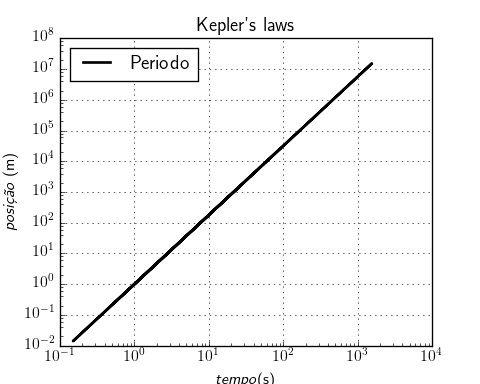
\includegraphics[width=4.80in,height=3.84in,keepaspectratio = false]{image1.png}
	
	\scriptsize Figura 2. O gráfico de $\log T$ versus $\log r$ para os dados planetários da Tabela 1.
	
\end{center}

\section{Conclu\c{c}\~ao}

Nesse trabalho deduzimos e verificamos a veracidade da 3$^\circ$ lei de kepler e que a relação entre o período e o raio da orbita dos planetas corre de forma logarítmica, e que as leis de Kepler e algo bem mais geral podendo descrever e prever o movimento de satélites.

\section{Referencia}

\noindent 

1)N. J. Giordano $\&$ H. Nakanishi, Computational Physics, 2ed, 2007

2)Sears $\&$ Zemansky, Física 2 Termodinâmica e ondas, 12ed, 2008

3)Talita A.Anjos, Brasil Escola,2016



\end{document}

